\section{Decomposition of Probability Distributions}\label{sec:prob_rep}

We here investigate tensor network decomposition mechanisms of probability distributions.
After introducing probability distributions as tensors we derive tensor network decompositions based on conditional independencies (applying the Hammersley-Clifford theorem \cite{clifford_markov_1971}) to motivate graphical models.
Further we present the \ComputationMechanism{}, in which the Fisher-Neyman Factorization Theorem is used to decompose distributions in the presence of sufficient statistics.

\subsection{Basic concepts}

Distributions $\probtensor$ over a discrete state space can be represented by tensors, where each entry corresponds to the probability of a corresponding state. The joint probability distribution for a set of categorical variables as in definition~\ref{def:atomic-factored-representation} is defined here.

\begin{definition}[Joint Probability Distribution]
    \label{def:probabilityDistribution} % From the axioms of Kolmogorov!
    Let there be for each $\catenumeratorin$ a categorical variable $\catvariableof{\catenumerator}$ taking values in $[\catdimof{\atomenumerator}]$.
    A joint probability distribution of these categorical variables is a function
    \begin{align*}
        \probwith \defcols \facstates \rightarrow \rr
    \end{align*}
    which is non-negative, that is for any $\shortcatindicesin$ it holds
    \begin{align*}
        \probat{\indexedshortcatvariables} \geq 0 \, ,
    \end{align*}
    and which is normalized, that is
    \begin{align*}
        \contraction{\probat{\shortcatvariables}} = 1 \, .
    \end{align*}
    Let $\thirdcatvariable$ be another variable taking values in a possibly infinite set $\mathrm{val}(\thirdcatvariable)$.
    Then a tensor $\condprobat{\shortcatvariables}{\thirdcatvariable}$ is a family of joint probability distributions, if for any $\thirdcatindex\in\mathrm{val}(\thirdcatvariable)$ the slice $\condprobat{\shortcatvariables}{\thirdcatvariable=\thirdcatindex}$ is a joint probability distribution.
\end{definition}

\begin{example}[Family of independent coin tosses]
    Consider tossing a coin with head probability $\thirdcatindex\in[0,1]$ and repeating the experiment independently $\catorder\in\nn$ times.
    We define a variable $\thirdcatvariable$ taking values in $\mathrm{val}(\thirdcatvariable)=[0,1]$ and denote by $\shortcatvariables$ $\catorder$ boolean variables.
    Then, the family of coin toss distributions is the tensor $\condprobat{\shortcatvariables}{\thirdcatvariable}$ with coordinates $\shortcatindices\in\atomstates$ and $\thirdcatindex\in[0,1]$ defined by
    \begin{align*}
        \condprobat{\indexedshortcatvariables}{\thirdcatvariable=\thirdcatindex}
        = \prod_{\catenumeratorin} \thirdcatindex^{\catindexof{\catenumerator}} (1-\thirdcatindex)^{1-\catindexof{\catenumerator}}
        = \thirdcatindex^{\sum_{\catenumeratorin} \catindexof{\catenumerator}} (1-\thirdcatindex)^{\catorder - \sum_{\catenumeratorin} \catindexof{\catenumerator}} \, .
    \end{align*}
    Note that for each slice with respect to $\thirdcatindex\in[0,1]$ by the binomial theorem we have $\contraction{\probat{\shortcatvariables,\thirdcatvariable=\thirdcatindex}}=1$ and thus $\probat{\shortcatvariables,\thirdcatvariable}$ is indeed a family of probability distributions.
    For $\catorder=2$ we have more explicitly for any $\thirdcatindex\in[0,1]$ that
    \begin{center}
        \begin{tikzpicture}[scale=1]
            \node[anchor=east] (A) at (-2,0) {$\condprobat{\catvariableof{[2]}}{\thirdcatvariable=\thirdcatindex}\,=$};

            \node (A) at (1,0) {
                $\begin{bmatrix}
                (1-\thirdcatindex)
                     ^2 & \thirdcatindex \cdot (1-\thirdcatindex) \\
                     \thirdcatindex \cdot (1-\thirdcatindex) & \thirdcatindex^2
                \end{bmatrix}$
            };
            \draw[<-,dashed] (-1.3,-0.275) node[right] {\tiny $1$} -- (-1.3,0.275) node [midway, left] {\tiny $\catvariableof{0}$} node[right] {\tiny $0$};
            \draw[->,dashed] (0,0.85) node[below] {\tiny $0$} -- (2,0.85) node [midway, above] {\tiny $\catvariableof{1}$} node[below] {\tiny $1$};
            \node[anchor=east] (A) at (3.5,-0.55) {$\cdot$};
        \end{tikzpicture}
    \end{center}
\end{example}

%\subsection{Reasoning based on contractions}

%\alex{The most central inference operation on probability distributions is the computation of marginals, which is just the contraction leaving only the marginalized variable open.
%Conditional probabilities are marginal proabilities of the distribution with added boolean tensors marking the evidence (e.g. one-hot encodings to states of some variables).
%With this formalism we can answer queries like "What is the probability of booking this account when having observed this feature on the invoice?".
%}

%\alex{Marginals are missing -> Add them and normalizations here!}

%In most of the analysis, we assume that every state in the space is assigned a positive probability.
%We say, a distribution $\probwith$ is \emph{positive} if $\mathbb{P}[X_{[d]} = x_{[d]}]>0$ for every configuration $x_{[d]}$.
%
%Note that in this tensor centered notation the calculation of marginal distributions reduces to contracting the open legs, not considered in the marginal with tensors $\ones$ only containing ones, see~\cite[Section 2.1.3]{goessmann_tensor-network_2025}.

A basic inference operation on probability distributions is the computation of marginal and conditional distribution. %, which is just the contraction leaving only the marginalized variable open.
%Conditional probabilities are marginal proabilities of the distribution with added boolean tensors marking the evidence (e.g. one-hot encodings to states of some variables).

\begin{definition}
    For any distribution $\probat{\catvariable,\seccatvariable}$ the marginal distribution is given by the contraction
    \begin{align*}
        \probat{\catvariable} \coloneqq \contractionof{\probat{\catvariable,\seccatvariable}}{\catvariable}
    \end{align*}
    which is depicted by the diagram
    \begin{center}
        \begin{tikzpicture}[scale=0.3,thick] % , baseline = -3.5pt

\draw (-19,-1) rectangle (-15,-3);
\node[anchor=center] (text) at (-17,-2) {\corelabelsize $\margprobat{\exrandom}$};
\draw[midarrow]  (-17,-3)--(-17,-5) node[midway,left] {\colorlabelsize $\exrandom$};

\node[anchor=center] (text) at (-13,-2) {${=}$};

\draw (-11,-1) rectangle (-5,-3);
\node[anchor=center] (text) at (-8,-2) {\corelabelsize $\probat{\exrandom,\secexrandom}$};
\draw[midarrow]  (-10,-3)--(-10,-5) node[midway,left] {\colorlabelsize $\exrandom$};
\draw[midarrow]  (-6,-3)--(-6,-5) node[midway,left] {\colorlabelsize $\secexrandom$};
\draw (-7,-5) rectangle (-5,-7); 
\node[anchor=center] (text) at (-6,-6) {$\ones$};

\end{tikzpicture}
    \end{center}
    The conditional distribution of $\catvariable$ on $\seccatvariable$ is a tensor $\condprobat{\catvariable}{\seccatvariable}$ defined for $\seccatindex\in[\catdimof{1}]$
    \begin{align*}
        \condprobat{\catvariable}{\seccatvariable=\seccatindex} \coloneqq
        \begin{cases}
            \frac{1}{\catdim} \cdot \onesat{\catvariable} & \ifspace \contraction{\probat{\catvariable,\seccatvariable=\seccatindex}} = 0 \\
            \frac{1}{\contraction{\probat{\catvariable,\seccatvariable=\seccatindex}}} \cdot \probat{\catvariable,\seccatvariable=\seccatindex} & \text{else}
        \end{cases} \,
    \end{align*}
    and in the second case depicted by the diagram
    \begin{center}
        \begin{tikzpicture}[scale=0.3, thick] % , baseline = -3.5pt

\draw (-21,-1) rectangle (-15,-3);
\node[anchor=center] (text) at (-18,-2) {\small $\condprobof{\exrandom}{\secexrandom}$};
\draw[->]  (-20,-3)--(-20,-5) node[midway,left] {\tiny $\exrandom$}; 

\draw[<-]  (-16,-3)--(-16,-5) node[midway,left] {\tiny $\secexrandom$}; 
\draw[dashed] (-15,-5) rectangle (-17,-7); 
\node[anchor=center] (text) at (-16,-6) {\small $\onehotmapof{\catindexof{\secexrandom}}$};

\node[anchor=center] (text) at (-13,-2) {${=}$};


\begin{scope}[shift={(0,6)}]

\draw (-11,-1) rectangle (-5,-3);
\node[anchor=center] (text) at (-8,-2) {\small $\probof{\exrandom,\secexrandom}$};
\draw[->]  (-10,-3)--(-10,-5) node[midway,left] {\tiny $\exrandom$}; 
\draw[->]  (-6,-3)--(-6,-5) node[midway,left] {\tiny $\secexrandom$};
\draw[dashed] (-7,-5) rectangle (-5,-7); 
\node[anchor=center] (text) at (-6,-6) {\small $\onehotmapof{\catindexof{\secexrandom}}$};

\end{scope}

\draw (-12,-2) -- (-4,-2);

\begin{scope}[shift={(0,-2)}]

\draw (-11,-1) rectangle (-5,-3);
\node[anchor=center] (text) at (-8,-2) {\small $\probof{\exrandom,\secexrandom}$};
\draw[->]  (-10,-3)--(-10,-5) node[midway,left] {\tiny $\exrandom$}; 
\draw (-11,-5) rectangle (-9,-7); 
\node[anchor=center] (text) at (-10,-6) {$\ones$};
\draw[->]  (-6,-3)--(-6,-5) node[midway,left] {\tiny $\secexrandom$};
\draw[dashed] (-7,-5) rectangle (-5,-7); 
\node[anchor=center] (text) at (-6,-6) {\small $\onehotmapof{\catindexof{\secexrandom}}$};

\end{scope}

\end{tikzpicture}
    \end{center}
\end{definition}


% \textcolor{gray}{One of them is by employing the chain rule.
% \begin{theorem}[Chain Rule]
%     \label{the:chainRule}
%     For any probability distribution $\probwith$ we have
%     \begin{align*}
%         \probat{\shortcatvariables}
%         = \contractionof{\{\margprobat{\catvariableof{0}}\} \cup
%         \left\{\condprobof{\catvariableof{\catenumerator}}{\catvariableof{0},\ldots,\catvariableof{\catenumerator-1}} \wcols \catenumeratorin \ncond \catenumerator\geq 1\right\}
%         }{\shortcatvariables} \, ,
%     \end{align*}
%     provided that all conditional probability distributions exist.
% \end{theorem}
% \textcolor{darkgray}{ graphical notation of chain rule/Markov chain?}
% In case of Markov chains, where each random variable only depends on the previous random variable, this leads to a efficient representation.
% In general, the chain rule does not lead to a complexity reduction as the distribution $\condprobof{\catvariableof{\catenumerator}}{\catvariableof{0},\ldots,\catvariableof{\catenumerator-1}}$ has the same dimensions as the original probability distribution $\probat{\shortcatvariables}$.
% Therefore, other decompositions can be considered.
% }
% \alex{Its important to note, that the chain rule for itself does not provide a more efficient representation of the distribution (since it is a generic decomposition). 
% To achieve efficient tensor network decomposition, one needs to combine that with conditional independence assumptions (as in the Markov Chain case), such that conditioned variables in the conditional probability distributions can be dropped.}

\subsection{The \IndependenceMechanism{}: Graphical Model Factorization}

%% Need for decomposition mechanisms: Motivation for independence considerations
The number of coordinates in a tensor representation of probability distributions is the product
\begin{align*}
    \prod_{\catenumeratorin}\catdimof{\catenumerator} \, ,
\end{align*}
and therefore scales exponentially in the number of coordinates.
To find efficient representation schemes of probability distributions by tensor networks, we need to exploit additional properties of the distribution.
%% Independence
Independence leads to severe sparsifications of conditional probabilities and is therefore the key assumption to gain sparse decompositions of probability distributions.

%Markov Networks on hypergraphs $\graph$ are exactly those \CompActNets{}, which are computable with respect to the identity and the graph $\graph$.
%We here show how the sets of Markov Networks can be characterized by conditional independence assumptions.
%\alex{We can present graphical models and independences as decomposition schemes of activation tensors.
%Usually in graphical models there are no computation cores, hence the "features" of the statistic are the same as the variables.
%In that case the activation tensor is the same as the joint distribution tensor, that is a contraction of tensors colored by subsets of the variables (building the edges of the graphical models).

\begin{definition}[Independence]
    \label{def:independence} %% Was {the:independenceProductCriterion} in the report!
    We say that $\catvariableof{0}$ is independent of $\catvariableof{1}$ with respect to a distribution $\probat{\catvariableof{0},\catvariableof{1}}$, if the distribution is the tensor product of the marginal distributions, that is
    \begin{align*}
        \probat{\catvariableof{0},\catvariableof{1}}
        = \probat{\catvariableof{0}} \otimes \probat{\catvariableof{1}} \, .
    \end{align*}
    In this case we denote $\independent{\catvariableof{0}}{\catvariableof{1}}$.
\end{definition}

Thus, independence appears directly as a tensor–product decomposition of probability distribution.
Using tensor network diagrams we depict this property by
\begin{center}
    \begin{tikzpicture}[scale=0.3,thick] % , baseline = -3.5pt


\draw (0,1) rectangle (7,-1);
\node[anchor=center] (text) at (3.5,0) {\corelabelsize $\probat{\exrandom,\secexrandom}$};
\draw[->-] (1,-1) -- (1,-3) node[midway, left] {\colorlabelsize $\exrandom$};
\draw[->-] (6,-1) -- (6,-3) node[midway, left] {\colorlabelsize $\secexrandom$};

\node[anchor=center] (text) at (9,0) {\corelabelsize ${=}$};


\begin{scope}[shift={(11,0)}]

\draw (0,1) rectangle (7,-1);
\node[anchor=center] (text) at (3.5,0) {\corelabelsize $\probat{\exrandom,\secexrandom}$};
\draw[->-] (1,-1) -- (1,-3) node[midway, left] {\colorlabelsize $\exrandom$};
\draw[->-] (6,-1) -- (6,-3) node[midway, left] {\colorlabelsize $\secexrandom$};
\draw (5,-3) rectangle (7,-5);
\node[anchor=center] (text) at (6,-4) {\corelabelsize $\ones$};

\end{scope}

\node[anchor=center] (text) at (20,0) {\corelabelsize $\otimes$};

\begin{scope}[shift={(22,0)}]

\draw (0,1) rectangle (7,-1);
\node[anchor=center] (text) at (3.5,0) {\corelabelsize $\probat{\exrandom,\secexrandom}$};
\draw[->-] (1,-1) -- (1,-3) node[midway, left] {\colorlabelsize $\exrandom$};
\draw (0,-3) rectangle (2,-5);
\node[anchor=center] (text) at (1,-4) {\corelabelsize $\ones$};
\draw[->-] (6,-1) -- (6,-3) node[midway, left] {\colorlabelsize $\secexrandom$};

\end{scope}

\node[anchor=center] (text) at (31,0) {\corelabelsize ${=}$};

\begin{scope}[shift={(33,0)}]

\draw (0,1) rectangle (4,-1);
\node[anchor=center] (text) at (2,0) {\corelabelsize $\margprobat{\exrandom}$};
\draw[->-] (2,-1) -- (2,-3) node[midway, left] {\colorlabelsize $\exrandom$};

\node[anchor=center] (text) at (6,0) {\corelabelsize $\otimes$};

\draw (8,1) rectangle (12,-1);
\node[anchor=center] (text) at (10,0) {\corelabelsize $\margprobat{\secexrandom}$};
\draw[->-] (10,-1) -- (10,-3) node[midway, left] {\colorlabelsize $\secexrandom$};


\end{scope}

\node[anchor=center] (text) at (46,-3) {\corelabelsize ${.}$};

\end{tikzpicture} 
\end{center}
Let us notice, that the assumption of independence reduces the degrees of freedom from $\exranddim\cdot\secexranddim-1$ to $(\exranddim-1)+(\secexranddim-1)$.
The decomposition into marginal distributions furthermore exploits this reduced freedom and provides an efficient storage.
Having a joint distribution of multiple variables, which disjoint subsets are independent, we can iteratively apply the decomposition scheme.
As a result, we can reduce the scaling of the degrees of freedom from exponential to linear by the assumption of independence.

Independence is, as we observed, a strong assumption, which is often too restrictive.
Conditional independence instead is a less demanding assumption, which still implies efficient tensor network decompositions schemes.
We introduce conditional independence as independence of variables with respect to conditional distributions.

\begin{definition}[Conditional Independence]
    \label{def:condIndependence} %% Was {the:condIndependenceProductCriterion} in the report!
    Given a joint distribution of variables $\catvariableof{0}$, $\catvariableof{1}$ and $\catvariableof{2}$, such that $\margprobat{\catvariableof{2}}$ is positive.
    We say that $\catvariableof{0}$ is independent of $\catvariableof{1}$ conditioned on $\catvariableof{2}$ if for any states $\exrandindin,\secexrandindin$ and $\thirdexrandindin$
    \begin{align*}
        \condprobof{\catvariableof{0},\catvariableof{1}}{\catvariableof{2}}
        = \contractionof{
            \condprobof{\catvariableof{0}}{\catvariableof{2}},\condprobof{\catvariableof{1}}{\catvariableof{2}}
        }{\catvariableof{0},\catvariableof{1},\catvariableof{2}} \, .
    \end{align*}
    In this case we denote $\condindependent{\catvariableof{0}}{\catvariableof{1}}{\catvariableof{2}}$.
\end{definition}

Conditional independence stated in \defref{def:condIndependence} has a close connection with independence stated in \defref{def:independence}.
To be more precise, $\catvariableof{0}$ is independent of $\catvariableof{1}$ conditioned on $\catvariableof{2}$, if and only if $\catvariableof{0}$ is independent of $\catvariableof{1}$ with respect to any slice $\condprobof{\catvariableof{0},\catvariableof{1}}{\indexedcatvariableof{2}}$ of the conditional distribution $\condprobof{\catvariableof{0},\catvariableof{1}}{\catvariableof{2}}$.

We can further exploit conditional independence to find tensor network decompositions of probabilities, as we show as the next corollary.
\begin{corollary}% NEEDED?
    \label{cor:secCriterionCondIndepencence}
    Let $\probat{\catvariableof{0},\catvariableof{1},\catvariableof{2}}$ be a joint distribution.
    If and only if $\catvariableof{0}$ is independent of $\catvariableof{1}$ conditioned on $\catvariableof{2}$ the distribution satisfies
    \begin{align*}
        \probat{\catvariableof{0},\catvariableof{1},\catvariableof{2}}
        = \contractionof{\condprobof{\catvariableof{0}}{\catvariableof{2}},\condprobof{\catvariableof{1}}{\catvariableof{2}},\margprobat{\catvariableof{2}}}{\catvariableof{0},\catvariableof{1},\catvariableof{2}} \, .
    \end{align*}
    In a diagrammatic notation this is depicted by
    \begin{center}
        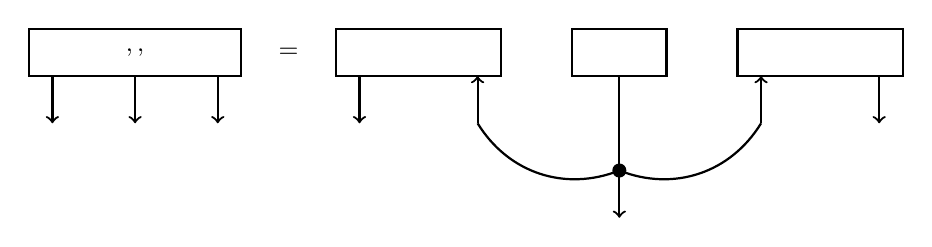
\begin{tikzpicture}[scale=0.3,thick] % , baseline = -3.5pt


\draw (-2,1) rectangle (7,-1);
\node[anchor=center] (text) at (2.5,0) {\small $\probof{\exrandom,\secexrandom,\thirdexrandom}$};
\draw[->] (-1,-1) -- (-1,-3) node[midway, left] {\tiny $\exrandom$};
\draw[->] (2.5,-1) -- (2.5,-3) node[midway, left] {\tiny $\secexrandom$};
\draw[->] (6,-1) -- (6,-3) node[midway, left] {\tiny $\thirdexrandom$};

\node[anchor=center] (text) at (9,0) {\small ${=}$};

\draw (11,1) rectangle (18,-1);
\node[anchor=center] (text) at (14.5,0) {\small $\condprobof{\exrandom}{\thirdexrandom}$};
\draw[->] (12,-1) -- (12,-3) node[midway, left] {\tiny $\exrandom$};
\draw[<-] (17,-1) -- (17,-3) node[midway, left] {\tiny $\thirdexrandom$};

\draw (21,1) rectangle (25,-1);
\node[anchor=center] (text) at (23,0) {\small $\probof{\thirdexrandom}$};
\draw (23,-1) -- (23,-3) node[midway, left] {\tiny $\thirdexrandom$};

\draw (23,-3) -- (23,-5);
\draw[fill] (23,-5) circle (0.25cm);
\draw[->] (23,-5) -- (23,-7) node[midway, left] {\tiny $\thirdexrandom$};
\draw (17,-3) to[bend right=40] (23,-5);
\draw (29,-3) to[bend right=-40] (23,-5);


\draw (28,1) rectangle (35,-1);
\node[anchor=center] (text) at (31.5,0) {\small $\condprobof{\secexrandom}{\thirdexrandom}$};
\draw[<-] (29,-1) -- (29,-3) node[midway, left] {\tiny $\thirdexrandom$};
\draw[->] (34,-1) -- (34,-3) node[midway, left] {\tiny $\secexrandom$};



\end{tikzpicture} 
    \end{center}
\end{corollary}

%\begin{figure}[t]
%    \begin{center}
%        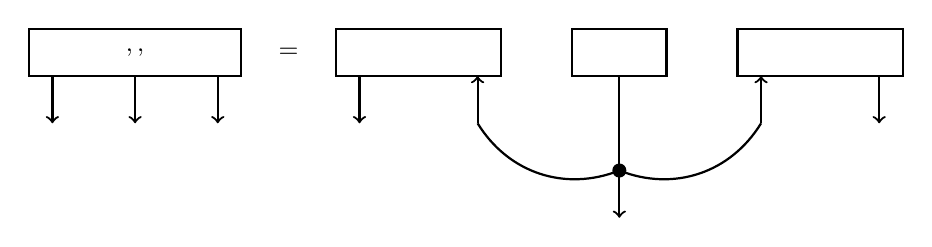
\begin{tikzpicture}[scale=0.3,thick] % , baseline = -3.5pt


\draw (-2,1) rectangle (7,-1);
\node[anchor=center] (text) at (2.5,0) {\small $\probof{\exrandom,\secexrandom,\thirdexrandom}$};
\draw[->] (-1,-1) -- (-1,-3) node[midway, left] {\tiny $\exrandom$};
\draw[->] (2.5,-1) -- (2.5,-3) node[midway, left] {\tiny $\secexrandom$};
\draw[->] (6,-1) -- (6,-3) node[midway, left] {\tiny $\thirdexrandom$};

\node[anchor=center] (text) at (9,0) {\small ${=}$};

\draw (11,1) rectangle (18,-1);
\node[anchor=center] (text) at (14.5,0) {\small $\condprobof{\exrandom}{\thirdexrandom}$};
\draw[->] (12,-1) -- (12,-3) node[midway, left] {\tiny $\exrandom$};
\draw[<-] (17,-1) -- (17,-3) node[midway, left] {\tiny $\thirdexrandom$};

\draw (21,1) rectangle (25,-1);
\node[anchor=center] (text) at (23,0) {\small $\probof{\thirdexrandom}$};
\draw (23,-1) -- (23,-3) node[midway, left] {\tiny $\thirdexrandom$};

\draw (23,-3) -- (23,-5);
\draw[fill] (23,-5) circle (0.25cm);
\draw[->] (23,-5) -- (23,-7) node[midway, left] {\tiny $\thirdexrandom$};
\draw (17,-3) to[bend right=40] (23,-5);
\draw (29,-3) to[bend right=-40] (23,-5);


\draw (28,1) rectangle (35,-1);
\node[anchor=center] (text) at (31.5,0) {\small $\condprobof{\secexrandom}{\thirdexrandom}$};
\draw[<-] (29,-1) -- (29,-3) node[midway, left] {\tiny $\thirdexrandom$};
\draw[->] (34,-1) -- (34,-3) node[midway, left] {\tiny $\secexrandom$};



\end{tikzpicture} 
%    \end{center}
%    \caption{Diagrammatic visualization of the contraction equation in \corref{cor:secCriterionCondIndepencence}.
%    Conditional independence of $\catvariableof{0}$ and $\catvariableof{1}$ given $\catvariableof{2}$ holds if the contraction on the right side is equal to the probability tensor on the left side.}
%    \label{fig:condIndependenceDecomposition}
%\end{figure}

%%% Repetition!
%By \theref{the:condIndependenceProductCriterion} and \corref{cor:secCriterionCondIndepencence}, the conditional independence $\catvariableof{0} \perp X_1 \mid X_2$ is equivalent to the factorization
%\[
%    \mathbb{P}[\catvariableof{0},X_1,X_2]
%    =
%    \bigl\langle
%    \mathbb{P}[\catvariableof{0}\mid X_2],\,\mathbb{P}[X_1\mid X_2],\,\mathbb{P}[X_2]
%    \bigr\rangle[\catvariableof{0},X_1,X_2],
%\]
%which is precisely the three–node graphical model with edges $(\catvariableof{0},X_1)$ and $(X_1,X_2)$ depicted in \figref{fig:condIndependenceDecomposition}.
%In the graphical–model CAN with identity statistic, the joint activation tensor $\xi[\catvariableof{0},X_1,X_2]$ thus decomposes into three smaller cores: a unary core on $X_2$ and two binary cores on $(\catvariableof{0},X_2)$ and $(X_1,X_2)$.


This conditional–independence pattern is the basic local building block that is generalized in Markov networks, which we define in the following.

\begin{definition}[Markov Network]
    \label{def:markovNetwork}
    Let $\tnetof{\graph}$ be a tensor network of non-negative tensors decorating a hypergraph $\graph$.
    Then the Markov Network $\probof{\graph}$ to $\tnetof{\graph}$ is the probability distribution of $\catvariableof{\node}$ defined by the tensor
    \begin{align*}
        \probofat{\graph}{\nodevariables} = \frac{
            \contractionof{\{\hypercoreof{\edge} \wcols \edgein\}}{\nodevariables}
        }{
            \contraction{\{\hypercoreof{\edge} \wcols \edgein\}}
        } = \normalizationof{\tnetof{\graph}}{\nodevariables} \, .
    \end{align*}
    We call the denominator
    \begin{align*}
        \partitionfunctionof{\tnetof{\graph}} = \contraction{\{\hypercoreof{\edge} \wcols \edgein\}}
    \end{align*}
    the partition function of the tensor network $\tnetof{\graph}$.
\end{definition}

We directly defined here graphical models on hypergraphs.
%% Graphical Models as Tensor Networks
It is known that probabilistic graphical models are dual to tensor networks \cite{robeva_duality_2019,glasser_expressive_2019}.
%By our hypergraph based definition of tensor networks, markov networks are equivalent to tensor networks of positive tensors.
We define graphical models based on hypergraphs, to establish a direct connection with tensor network decorating the hypergraph.
In a more canonical way, Markov Networks are instead defined by graphs, where instead of the edges the cliques are decorated by factor tensors (see for example \cite{koller_probabilistic_2009}).

%% CompActNets as Markov Networks - Check for redundancy!
We can interpret the factors $\hypercorewith$ as activation cores placed on the hyperedges $\edge$ of the graph.
The global activation tensor (and hence the joint distribution) is obtained by contracting this activation network and normalizing by its partition function.

%We call $\probwith$ \emph{positive} if $\probat{\indexedshortcatvariables}> 0$ for all states $\shortcatindices$.
%The marginalization of a Markov Network to $\tnetof{\graph}$ on subsets of variables $\catvariableof{\secnodes}$ is
%\begin{align*}
%    \probofat{\graph}{\catvariableof{\secnodes}}
%    = \normalizationof{\tnetof{\graph}}{\catvariableof{\secnodes}} \, .
%\end{align*}

%This can be derived from a commutativity of contractions, which established an equivalence of contractions with sequences of consecutive contractions.
%\begin{theorem}[Commutativity of Contractions] % NEEDED?
%    \label{the:splittingContractions}
%    Let $\tnetof{\graph}$ be a tensor network on a hypergraph $\graph=(\nodes,\edges)$.
%    Let us now split the $\graph$ into two graphs $\graph_1=(\nodesone,\edges_1)$ and $\graph_2=(\nodestwo,\edges_2)$, such that $\edges_1\dot{\cup}\edges_2=\edges$, $\nodesone\cup\nodestwo=\nodes$ and all nodes in $\nodestwo$ are contained in an hyperedge of $\edges_2$.
%    We then have for any $\secnodes\subset\nodes$
%    \begin{align*}
%        \contractionof{\tnetof{\graph}}{\catvariableof{\secnodes}}
%        = \contractionof{
%            \tnetofat{\graph_1}{\catvariableof{\nodesone}}
%            \cup \{\contractionof{\tnetof{\graph_2}}{\catvariableof{\nodestwo\cap(\nodesone\cup\secnodes)}}\}
%        }{\catvariableof{\secnodes}}   \, .
%    \end{align*}
%\end{theorem}

%Further, the distribution of $\catvariableof{\secnodes}$ conditioned on $\catvariableof{\thirdnodes}$, where $\secnodes,\thirdnodes$ are disjoint subsets of $\nodes$, is
%\begin{align*}
%    \probtensor^{\graph}\left[\catvariableof{\secnodes}|\catvariableof{\thirdnodes}\right]
%    = \normalizationofwrt{\tnetof{\graph}}{\catvariableof{\secnodes}}{\catvariableof{\thirdnodes}} \, .
%\end{align*}

While we have directly defined Markov Networks as decomposed probability distributions, we now want to derive assumptions on a distribution assuring that such decompositions exist.
As we will see, the sets of conditional independencies encoded by a hypergraph are captured by its seperation properties, as we define next.

\begin{definition}[Separation of Hypergraph]
    A path in a hypergraph is a sequence of nodes $\node_{\atomenumerator}$ for $\atomenumeratorin$, such that for any $\atomenumerator\in[\atomorder-1]$ we find a hyperedge $\edgein$ such that $(\node_{\atomenumerator}, \node_{\atomenumerator+1})\subset \edge$.
    Given disjoint subsets $\nodesa$, $\nodesb$, $\nodesc$ of nodes in a hypergraph $\graph$ we say that $\nodesc$ separates $\nodesa$ and $\nodesb$ with respect to $\graph$, when any path starting at a node in $\nodesa$ and ending in a node in $\nodesb$ contains a node in $\nodesc$.
\end{definition}

To characterize Markov Networks in terms of conditional independencies we need to further define the property of clique-capturing.
This property of clique-capturing established a correspondence of hyperedges with maximal cliques in the more canonical graph-based definition of Markov Networks \cite{koller_probabilistic_2009}.

\begin{definition}[Clique-Capturing Hypergraph]
    \label{def:ccHypergraph}
    We call a hypergraph $\graph$ clique-capturing, when each subset $\secnodes\subset\nodes$ is contained in a hyperedge, if for any $a,b\in\secnodes$ there is a hyperedge $\edgein$ with $a,b\in\secnodes$.
\end{definition}

Let us now show a characterization of Markov Networks in terms of conditional independencies.

% Characterization
\begin{theorem}[Hammersley-Clifford Factorization Theorem]
    \label{the:factorizationHammersleyClifford}
    Given a clique-capturing hypergraph $\graph$, the set of positive Markov Networks on the hypergraph coincides with the set of positive probability distributions, such that for each disjoint subsets of variables $\nodesa$, $\nodesb$, $\nodesc$ we have $\catvariableof{\nodesa}$ is independent of $\catvariableof{\nodesb}$ conditioned on $\catvariableof{\nodesc}$, when $\nodesc$ separates $\nodesa$ and $\nodesb$ in the hypergraph. % called d-separation
\end{theorem}
\begin{proof}
    Shown in Appendix~\secref{sec:proofFactorizationTheorems}.
\end{proof}


\begin{example}[I.i.d. Boolean Variables: Coin toss interpretation]\label{exa:ctHc}
    Let there be $\catorder$ boolean variables $\shortcatvariables$, which are i.i.d. drawn from a positive distribution $\probat{\catvariable}$.
    From the pairwise independencies of $\catvariableof{\catenumerator}$ it follows with the Hammersley-Clifford Factorization Theorem that the distribution is representable by an elementary tensor network, that is
    \begin{align*}
        \probwith = \bigotimes_{\catenumeratorin} \probat{\catvariableof{\catenumerator}} \, .
    \end{align*}
\end{example}


Equivalently, \theref{the:factorizationHammersleyClifford} states that for any strictly positive joint distribution $\mathbb{P}[X_V]$ whose conditional independencies are exactly those encoded by a clique–capturing hypergraph $G=(V,E)$, there exist non–negative activation cores $\tau_e[X_e]$ such that
\[
    P[X_V]
    =
    \frac{1}{Z}\,
    \contractionof{}{}
    \bigl\langle \{\tau_e : e \in E(G)\} \bigr\rangle[X_V],
\]
for a suitable normalizing constant $Z>0$.
Thus, the conditional–independence structure of $\mathbb{P}$ determines a global tensor–network decomposition of its activation (and hence joint) tensor.
We refer to this correspondence between independence structure and tensor–network factorization as the \emph{independence mechanism}, in analogy to the computation mechanism provided by sufficient statistics in Section 3.1.

\subsection{The \ComputationMechanism{}: Factorization in presense of Sufficient Statistics}
%\subsection{Sufficient statistics leading to tensor network decompositions ("the computation mechanism")}

\begin{definition}
    \label{def:sufStatistic}
    Let $\probat{\catvariable,\thirdcatvariable}$ be a joint distribution of the $\catdim$-dimensional variable $\catvariable$ and the $\thirdcatdim$-dimensional variable $\thirdcatvariable$ and let
    \begin{align*}
        \sstat \defcols [\catdim] \rightarrow [\headdim]
    \end{align*}
    be a statistic.
    We are interested in the distribution $\probat{\catvariable,\thirdcatvariable,\headvariableof{\sstat}}=\contractionof{\probat{\catvariable,\thirdcatvariable},\bencodingofat{\sstat}{\headvariableof{\sstat},\catvariable}}{\catvariable,\thirdcatvariable,\headvariableof{\sstat}}$.
    We say that $\sstat$ is a sufficient statistic for $\thirdcatvariable$ if and only if $\catvariable$ is independent of $\thirdcatvariable$ conditioned on $\headvariableof{\sstat}$.
\end{definition}

Note that the independence in \defref{def:sufStatistic} is true if and only if
\begin{align*}
    \condprobat{\catvariable}{\thirdcatvariable,\headvariableof{\sstat}}
    =   \condprobat{\catvariable}{\headvariableof{\sstat}} \otimes \onesat{\thirdcatvariable} \, .
\end{align*}

\begin{example}[Sufficient Statistics for the Probability]\label{exa:sufStatProb}
    Let $\thirdcatvariable$ be the value $\probat{\indexedshortcatvariables}$, when drawing $\shortcatvariables$ from $\probwith$.
    Then $\sstat$ is a sufficient statistic for $\thirdcatvariable=\probwith$, if for all $\headindex$ in the image of $\sstat$ we have
    \begin{align*}
        \condprobof{\indexedshortcatvariables}{\sstatat{\shortcatindices}=\headindex} =
        \begin{cases}
            \frac{1}{\cardof{\{\shortcatindices \wcols \sstatat{\shortcatindices}=\headindex\}}} & \ifspace \sstat(\shortcatindices)=\headindex \\
            0 & \text{else}
        \end{cases} \, .
    \end{align*}
    %% Explanation
    When knowing the value $\sstat{\shortcatindices}$ of the sufficient statistic at a given index $\shortcatindices$, we then also know the probability $\probat{\indexedshortcatvariables}$.
    %% Old {the:sufficientStatisticActCoreExistence}
    The function $\sstat$ is thus a sufficient statistic for $\thirdcatvariable=\probwith$, if and only if there is a tensor $\acttensorwith$ with
    \begin{align*}
        \probat{\shortcatvariables}
        = \contractionof{\bencodingofat{\sstat}{\headvariables,\shortcatvariables},\acttensorwith}{\shortcatvariables} \, .
    \end{align*}
\end{example}

\exaref{exa:sufStatProb} hints at a connection between sufficient statistics and decompositions into \CompActNets{}.
More generally, such decompositions are provided by the Fisher-Neyman Factorization Theorem.

\begin{theorem}[Fisher-Neyman Factorization Theorem] % See appendix of CompAct Nets paper!
    \label{the:factorizationFisherNeyman}
    Let $\probtensor$ be a joint distribution of variables $\catvariable,\thirdcatvariable$ with values $\mathrm{val}(\catvariable), \,\mathrm{val}(\thirdcatvariable)$.
    Let there further be a finite set $\mathrm{val}(\headvariableof{\sstat})$.
    Then $\sstat\defcols \mathrm{val}(\catvariable) \rightarrow \mathrm{val}(\headvariableof{\sstat})$ is a sufficient statistic for $\thirdcatvariable$ if and only if there are tensors $\basemeasureat{\catvariable}$ and $\acttensorat{\headvariableof{\sstat},\thirdcatvariable}$ such that
    \begin{align*}
        \probat{\catvariable,\thirdcatvariable}
        = \contractionof{
            \acttensorat{\headvariableof{\sstat},\thirdcatvariable}\bencodingofat{\sstat}{\headvariableof{\sstat},\catvariable},\basemeasureat{\catvariable}
        }{\catvariable,\thirdcatvariable} \, .
    \end{align*}
    We depict this equation diagrammatically by
    \begin{center}
        \begin{tikzpicture}[scale = 0.35, thick]

    \draw (1,-1) rectangle (8,-4);
    \node[anchor=center] (text) at (4.5,-2.5) {\corelabelsize $\probtensor$};
    \draw (2.5,-4) -- (2.5,-6) node[midway, left] {\colorlabelsize $X$};
    \draw (6.5,-4) -- (6.5,-6) node[midway, right] {\colorlabelsize $Z$};

    \node[anchor=center] (text) at (10,-2.5) {${=}$};

    \begin{scope}[shift={(15,0)}]

        \draw (-3.5,-0.5) rectangle (-0.5,2.5);
        \node[anchor=center] (text) at (-2,1) {\corelabelsize $h$};
        \draw (-2,-0.5) -- (-2,-4);
        \draw (-2,-4) -- (-2,-6) node[midway, left] {\colorlabelsize $Z$};

        \drawvariabledot{-2}{-2.5}
        \draw[] (-2,-2.5) -- (0,-2.5);
        \draw[->-] (-1.5,-2.5) -- (0,-2.5);
        \draw (0,-1) rectangle (3,-4);
        \node[anchor=center] (text) at (1.5,-2.5) {\corelabelsize $\bencodingof{T}$};

        \draw[->-] (3,-2.5) -- (4.5,-2.5);
        \drawvariabledot{4.25}{-2.5}
        \draw[] (3,-2.5) -- (5,-2.5) node[midway, below] {\colorlabelsize $\headvariableof{T}$};

        \draw (5,-1) rectangle (8,-4);
        \node[anchor=center] (text) at (6.5,-2.5) {\corelabelsize $g$};
        \draw (6.5,-4) -- (6.5,-6) node[midway, right] {\colorlabelsize $X$};
    \end{scope}
\end{tikzpicture}
    \end{center}
\end{theorem}
\begin{proof}
    Shown in more generality in the appendix, see \theref{the:generalFactorizationFisherNeyman}.
\end{proof}

%%
Notice, that the definition of sufficient statistic does not make use of the marginal distribution $\probat{\thirdcatvariable}$.
We therefore can define sufficient statistics also for families of distributions $\condprobat{\catvariable}{\thirdcatvariable}$, with respect to arbitrary non-degenerate marginal distribution $\probat{\thirdcatvariable}$.
We then use the \theref{the:factorizationFisherNeyman} to embed such families in \CompActNets{}.

\begin{corollary}
    Let $\condprobof{\shortcatvariables}{\thirdcatvariable}$ be an arbitrary family of distributions of $\shortcatvariables$, which is .
    Then there is a tensor $\basemeasurewith$ and a activation tensors $\acttensorat{\headvariables,\thirdcatvariable}$ such that for any $\thirdcatindex\in\mathrm{val}(\thirdcatvariable)$
    \begin{align*}
        \condprobat{\shortcatvariables}{\thirdcatvariable=\thirdcatindex} \in\cansof{\sstat,\maxgraph,\basemeasure} \, .
    \end{align*}
\end{corollary}

\begin{example}[Order Statistic for Boolean Variables: Coin toss interpretation]\label{exa:coinToss}
    Let there be $\catorder$ boolean variables $\shortcatvariables$ and a family $\{\probofat{\theta}{\shortcatvariables}\wcols\theta\in\Theta\}$ of distributions.
    The order statistic assigns to each tuple $\shortcatindices$ the ordered tuple, which effectively counts the number of $1$ coordinates in the tuple $\shortcatindices$, that is the statistic
    \begin{align*}
        \sstatof{+} \defcols \facstates \rightarrow [\seldim] \quad, \quad \sstatof{+}(\shortcatindices) = \cardof{\{\catenumerator \wcols \catindexof{\catenumerator}=1\}} \, .
    \end{align*}
    When the order statistic is sufficient, the detailed order of the outcomes is uninformative about the member $\theta\in\Theta$ from which the random variables have been drawn.
    Let us now investigate those families for which $\sstatof{+}$ is a sufficient statistic.
    By the Fisher-Neyman Factorization Theorem \theref{the:factorizationFisherNeyman} $\sstatof{+}$ is a sufficient statistic if and only if there are tensors $\basemeasurewith$ and $\acttensorat{\headvariableof{+},\Theta}$ such that for each $\theta\in\Theta$
    \begin{align*}
        \probofat{\theta}{\shortcatvariables}
        = \contractionof{
            \acttensorofat{\theta}{\headvariableof{+}},\bencodingofat{\sstatof{+}}{\headvariableof{+},\shortcatvariables},\basemeasurewith}{\shortcatvariables} \, .
    \end{align*}

    The family of distributions, such that the variables $\shortcatvariables$ are i.i.d. with respect to each (see \exaref{exa:ctHc}) are the special case, where $\basemeasurewith=\onesat{\shortcatvariables}$ and the family is labeled by $\theta\in[0,1]$ such that for $\theta\in(0,1)$ and $\catenumerator\in[\catorder+1]$
    \begin{align*}
        \acttensorofat{\theta}{\headvariableof{+}=\catenumerator}
        = (1-\theta)^{\catorder-\catenumerator} \cdot \theta^{\catenumerator} \, ,
    \end{align*}
    and for $\theta\in\{0,1\}$
    \begin{align*}
        \acttensorofat{\theta}{\headvariableof{+}}  = \begin{cases}
                                                          \onehotmapofat{0}{\headvariableof{+}} & \ifspace \theta=0 \\
                                                          \onehotmapofat{\catorder}{\headvariableof{+}} & \ifspace \theta=1
        \end{cases}\, .
    \end{align*}
    The marginal distribution $\probofat{\theta}{\headvariableof{+}}$ is then the binominal distribution $B(\catorder,\theta)$.

%    We further notce, that
%    \begin{align*}
%        \contractionof{}{}
%    \end{align*}
%    If the base measure $\basemeasurewith$ itself is elementary, we have a coin toss family, if the order statistic is sufficient for the probability.
%
%
%    For the case $\catorder=2$:
%    Consider two coin tosses \(\catvariableof{0},\catvariableof{1}\in\{0,1\}\) (1=heads). With $p \in [0,1]$ being the probability of heads. Define the statistic
%    \[
%        S(X_1,X_2)=X_1+X_2\in\{0,1,2\}.
%    \]
%    Intuitively, \(S\) forgets order and keeps only the \emph{number of heads}. The conditional law of the sequence given \(S\) is uniform over all sequences with that many heads:
%    \[
%        \mathbb{P}\!\big((X_1,X_2)=(x_1,x_2)\mid S=k\big)=\frac{1}{\binom{2}{k}}
%        \quad\text{whenever }x_1+x_2=k.
%    \]
%    Thus, knowing \(S\) renders the detailed order uninformative about the distribution—this matches the idea of a \emph{sufficient statistic}.
%
%%\end{example}
%%\begin{example}{}
%
%    % Unfair and dependent coin toss — Factorization as a \ComputationActivationNetwork{}
%    Let \(X_1,X_2\in\{0,1\}\) and define the statistic \(S(X_1,X_2)=X_1+X_2\in\{0,1,2\}\).
%    The \emph{basis (computation) core} for this statistic is
%    \[
%        \beta_S[y,x_1,x_2]\;=\;\mathbf{1}\{\,y=x_1+x_2\,\},\qquad y\in\{0,1,2\}.
%    \]
%    For $p \in (0,1)$, define a \emph{unary activation} (a vector) \(\xi[Y]\) with components \(\xi[0]=(1-p)^2,\ \xi[1]=(1-p)p,\ \xi[2]=p^2\).
%    The joint distribution factors as
%    \[
%        \mathbb{P}[X_1,X_2]\;=\;\frac{1}{Z}\,\big\langle \beta_S[Y,X_1,X_2],\,\xi[Y]\big\rangle_{Y}
%    \]
%    with
%    \begin{align*}
%        Z&\coloneqq\big\langle\,\big\langle \beta_S[Y,X_1,X_2],\,\xi[Y]\big\rangle_Y\,\big\rangle_{[\varnothing]}\\
%        &=\sum_{y=0}^{2}\xi[y]\sum_{x_1=0}^1\sum_{x_2=0}^1\beta_S[y,x_1,x_2] = 1\xi[0] + 2\xi[1] + 1\xi[2]\\
%        &= (1-p)^2+2(1-p)p+p^2 = (p+ (1-p))^2 = 1
%    \end{align*}
%    Equivalently, in coordinates,
%    \[
%        \mathbb{P}[x_1,x_2]
%        \;=\;\frac{1}{Z}\sum_{y=0}^{2}\beta_S[y,x_1,x_2]\;\xi[y]
%        \;=\;\xi\!\big(S(x_1,x_2)\big).
%    \]
%
%% \medskip
%% \noindent\emph{Numerics for \(\xi=[1,1,1]\).}
%    Since \(S(0,0)=0\), \(S(0,1)=S(1,0)=1\), and \(S(1,1)=2\),
%% the unnormalized probabilities are
%% \[
%% \mathbb{P}^\star[0,0]=1,\quad \mathbb{P}^\star[0,1]=1,\quad \mathbb{P}^\star[1,0]=1,\quad \mathbb{P}^\star[1,1]=1,
%% \]
%% hence \(Z=\sum \mathbb{P}^\star=4\) and
%% \[
%% \mathbb{P}=
%% \begin{array}{c|cc}
%%  & X_2=0 & X_2=1\\\hline
%% X_1=0 & 1/4 & 1/4\\
%% X_1=1 & 1/4 & 1/4
%% \end{array}
%% \]
%    the induced law of the statistic is
%    \[
%        \mathbb{P}[S=0]=(1-p)^2,\qquad \mathbb{P}[S=1]=2p(1-p),\qquad \mathbb{P}[S=2]=p^2,
%    \]
%    reflecting that there is only one configuration for $y \in \{0,2\}$ and 2 configurations for $ y=1$.
\end{example}

The Fisher-Neyman Theorem is the fundamental motivation for the \CompActNets{} Architecture:
\begin{itemize}
    \item The tensors in a decomposition of $\acttensorwith$ are called \emph{activation cores}.
    \item The tensors in a decomposition of $\bencodingofat{\sstat}{\headvariables,\shortcatvariables}$ are called \emph{computation cores}.
\end{itemize}

\begin{example}[Graphical Models as a special case of \CompActNets{}]
    Recall \defref{def:realizableStatDistributions}.
    Given a statistic $\sstat:\facstates \to \parspace$ and a hypergraph $\graph=(\nodes,\edges)$ on the image coordinates $\headvariables$, any by $\sstat$ computable and by $\graph$ activated \CompActNets{} has the form
    \begin{align*}
        \probwith =  \normalizationof{\acttensorwith,\bencsstatwith}{\shortcatvariables}
    \end{align*}
    where $\acttensorwith$ is an arbitrary non-negative tensor.
    For graphical models we take the \emph{identity statistic}
    \[
        \identity\big(\shortcatindices\big)
        = \shortcatindices,
    \]
    so that the image coordinates coincide with the variables and there are no non-trivial computation cores.
    The associated basis encoding is just the identity tensor
    \begin{align*}
        \bencodingofat{\identity}{\headvariableof{[\catorder]},\shortcatvariables} = \identityat{\shortcatvariables,\headvariableof{[\catorder]}} \, .
    \end{align*}
    and therefore, for any activation tensor $\xi[Y[d]]$ we obtain
    \begin{align*}
        \probwith
        &= \normalizationof{\acttensorwith,\bencodingofat{\identity}{\headvariableof{[\catorder]},\shortcatvariables}}{\shortcatvariables}
        & = \normalizationof{\acttensorat{\shortcatvariables}}{\shortcatvariables}
    \end{align*}
    In other words, in the graphical–model case the activation tensor coincides with the joint distribution tensor.
    In this setting, structural properties of the distribution such as (conditional) independences can be read off as algebraic factorization patterns of the activation (and hence joint) tensor.

\end{example}

\subsection{Exponential families in case of elementary activation tensors}

% Universal properties
A classical theorem by Pitman-Koopman-Darmois (see \cite{pitman_sufficient_1936}) states, that whenever a family with constant support and a finite sufficient statistic for arbitrary large data sets is in an exponential family.
We now restrict the activation cores to specific elementary tensors, which correspond with further assumptions on the dependence of $\probtensor$ and $\sstat$ made by exponential families.
For a discussion of further universal properties of exponential families, such that the existence of priors and entropy maximizers, see \cite{murphy_probabilistic_2022}.

\begin{definition}[Exponential Family]
    %\alex{was \theref{the:expFamilyTensorRep}}
    Given a base measure $\basemeasure$ and a statistic $\sstat:\facstates\rightarrow\parspace$ we enumerate for each coordinate $\selindexin$ the image $\imageof{\sstatcoordinateof{\selindex}}$ by an interpretation map
    \begin{align*}
        \indexinterpretationof{\selindex} \defcols
        [\cardof{\imageof{\sstatcoordinateof{\selindex}}}] \rightarrow \imageof{\sstatcoordinateof{\selindex}} \, .
    \end{align*}
    For any canonical parameter vector $\canparamwithin$ we build the activation cores $\softactlegwith$ for each coordinate $\headindexof{\selindex}\in[\cardof{\imageof{\sstatcoordinateof{\selindex}}}]$ by
    \begin{align*}
        \softactlegat{\indexedheadvariableof{\selindex}}
        = \expof{\canparamat{\indexedselvariable} \cdot \indexinterpretationofat{\selindex}{\headindexof{\selindex}}} \,
    \end{align*}
    and define the distribution % Could do parametrization to thirdcatvariable to make connection with the family definition..
    \begin{align*}
        \expdistwith =
        \normalizationof{\{\basemeasurewith\} \cup \{\bencodingofat{\sstatcoordinateof{\selindex}}{\headvariableof{\selindex},\shortcatvariables} \wcols \selindexin\}\cup\{\softactlegwith \wcols \selindexin\}}{\shortcatvariables} \, .
    \end{align*}
    We then call the tensor $\probfamilyofat{\sstat,\basemeasure}{\shortcatvariables}{\Theta}$ with $\valof{\Theta}=\parspace$ and slices for $\canparamin$ by
    \begin{align*}
        \probfamilyofat{\sstat,\basemeasure}{\shortcatvariables}{\Theta=\canparam}
        = \expdistwith
    \end{align*}
    the exponential family to the statistic $\sstat$ and the base measure $\basemeasure$.
\end{definition}

%% In Elementary Activations
Note that by construction each member of an exponential family is an element in a \CompActNet{} with elementary activation cores (see \defref{def:elementaryActivation}), that is
\begin{align*}
    \probfamilyofat{\sstat,\basemeasure}{\shortcatvariables}{\Theta=\canparam}
    \in \cansof{\sstat,\elgraph,\basemeasure} \, .
\end{align*}

\begin{figure}
    \begin{center}
        \input{/Users/goessmann/Documents/tnreason/notes/summaries/computation_activation/tikz_pics/probability_representation/expdist_elementary}
    \end{center}
    \caption{
        Tensor Network diagram of a member of an exponential family $\probfamilyofat{\sstat,\basemeasure}{\shortcatvariables}{\Theta=\canparam}$ before normalization as an \CompActNet{} with elementary activation, that is an element in $\cansof{\sstat,\elgraph,\basemeasure}$.}\label{fig:expdistElementary}
\end{figure}

\begin{example}[Joint distributions of two booleans]
%{\alex{Joint distributions of two Booleans, sufficient statistic by head count (coin toss interpretation) and exponential family in case of independence}}
    In general, joint distribution of two Boolean variables $\catvariableof{0},\catvariableof{1}$ are 2x2 matrices of non-negative coordinates summing to 1:
    \[
        \probat{\catvariableof{[2]}}= \begin{bmatrix}
                                  p_{0,0} & p_{0,1} \\
                                  p_{1,0} & p_{1,1}
        \end{bmatrix}
    \]
    In the following example, we will assume at different points that $\catvariableof{0},\catvariableof{1}$ have a sufficient statistic, are independent and they have positive distributions.
    By the normalization constraint, $p_{1,1}$ is determined from $p_{0,0},p_{0,1}$ and $p_{1,0}$, which leaves us with three free parameters.
    \[
        \probat{\catvariableof{[2]}}= \begin{bmatrix}
                                  p_{0,0} & p_{0,1} \\
                                  p_{1,0} & 1-(p_{0,0}+p_{0,1}+p_{1,0})
        \end{bmatrix}
    \]

    Let us now restrict to those distributions, which have the sum $\catvariableof{0}+\catvariableof{1}$ as a sufficient statistic.
    They need to satisfy $p_{0,1}=p_{1,0}$ (since in that cases the statistic is 1 and the definition of sufficiency is that the distribution conditioned on the statistic is uniform), leaving us with two free parameters.
    \[
        \probat{\catvariableof{[2]}}= \begin{bmatrix}
                                  p_{0,0} & p_{0,1} \\
                                  p_{0,1} & 1-p_{0,0}-2p_{0,1}
        \end{bmatrix}
    \]
    This symmetry also implies, that the distributions are identically distributed, i.e. for any $\catindex\in\{0,1\}$ we have % with $\mathbb{I}_2 = (1,1)^\intercal$:
    \begin{align*}
        \probat{\catvariableof{0}=\catindex}
        = \contractionof{\probat{\catvariableof{0},\catvariableof{1}}}{\catvariableof{0}=\catindex}
        = \contractionof{\probat{\catvariableof{1},\catvariableof{0}}}{\catvariableof{1}=\catindex}
        = \probat{\catvariableof{1}=\catindex} \, .
    \end{align*}
%    \[
%        \probat{\catvariableof{0}}
%        = \left\langle \probat{\catvariableof{0},\catvariableof{1}}, \mathbb{I}[\catvariableof{1}] \right\rangle[\catvariableof{0}] = \probat{\catvariableof{0},\catvariableof{1}}\mathbb{I}_2 = \probat{\catvariableof{1},\catvariableof{0}} \mathbb{I}_2 = \left\langle \probat{\catvariableof{0},\catvariableof{1}}, \mathbb{I}[\catvariableof{0}] \right\rangle[\catvariableof{1}]
%        =\probat{\catvariableof{1}}.
%    \]

    Restricting further to those, where $\catvariableof{0}$ and $\catvariableof{1}$ are independent and the distribution is everywhere supported, brings us to the rank one formulation of the distribution
    \[
        \probat{\catvariableof{0},\catvariableof{1}} = \begin{bmatrix}
                               \probat{\catvariableof{0}=0}\probat{\catvariableof{1}=0} & \probat{\catvariableof{0}=0}\probat{\catvariableof{1}=1}\\
                               \probat{\catvariableof{0}=1}\probat{\catvariableof{1}=0} & \probat{\catvariableof{0}=1}\probat{\catvariableof{1}=1}
        \end{bmatrix} = \probat{\catvariableof{0}} \otimes \probat{\catvariableof{1}} %= \probat{\catvariableof{0}}\probat{\catvariableof{0}}^\intercal.
    \]
    In terms of an exponential family with the head count as a sufficient statistic, we parametrize the distribution by the canonical parameter $\canparam\in\rr$ as
    \[
        \probat{\catvariableof{0}}
        =\frac{1}{1+\expof{\canparam}}
        \begin{bmatrix}
            1 \\
            \expof{\canparam}
        \end{bmatrix}
    \]
    Note, that with this parametrization the probabilities for head and tail automatically have the form $p, (1-p)$.
    \[
        % \frac{1}{1+2\cdot\expof{\canparam}+\expof{2\canparam}}
        %     \begin{bmatrix}
        %         1 & \expof{\canparam} \\
        %         \expof{\canparam} & \expof{2\canparam}
        %     \end{bmatrix}
        % =
        \probat{\catvariableof{0},\catvariableof{1}} = \frac{1}{(1+\expof{\canparam})^2} \begin{bmatrix}
                                                                 1 \\
                                                                 \expof{\canparam}
        \end{bmatrix}
        \begin{bmatrix}
            1 &  \expof{\canparam}
        \end{bmatrix}
    \]
    % Furthermore, from the decomposition on the right side we see that $\catvariableof{0}$ and $\catvariableof{1}$ are independent.
    % Conversely, if $\catvariableof{0}$ and $\catvariableof{1}$ are independent and the distribution has the head count as sufficient statistic, $\catvariableof{0}$ and $\catvariableof{1}$ need to also be identical distributed (otherwise we would have $p_{0,1}\neq p_{1,0}$).
    % Using that the support is maximal, we find a $\canparam\in\rr$ such that 


    % and their joint distribution is the member of the exponential family to this parameter $\canparam$.

    %% SEE EXAMPLE 5.5 in [Lehmann Casella - Theory of Point Estimation]
    We can interpret this distribution as two independent coin tosses with outcome $\catvariableof{0}$ and $\catvariableof{1}$ and head probability
    \begin{align*}
        \probat{\catvariableof{0}=1} = \probat{\catvariableof{1}=1} = \frac{\expof{\canparam}}{1+\expof{\canparam}}
    \end{align*}
    which is the sigmoid of $\canparam$ and inverted by the logit
    \begin{align*}
        \canparam = \lnof{\frac{\probat{\catvariableof{0}=1}}{1-\probat{\catvariableof{0}=1}}} \, .
    \end{align*}
    Consistent with the above parametrization, we have a uniform distribution of $\catvariableof{0}$ and $\catvariableof{1}$ in the fair coin toss case $\probat{\catvariableof{0}=1}=0.5$, where $\canparam=0$.

    As a \ComputationActivationNetwork{} we can represent any distribution $\probat{\catvariableof{0},\catvariableof{1}}$ with the head count $+$ as sufficient statistic by
    \begin{align*}
        \probat{\catvariableof{0},\catvariableof{1}}
        &= \normalizationof{\bencodingofat{+}{\headvariableof{+},\catvariableof{0},\catvariableof{1}},\acttensorat{\headvariableof{+}}}{\catvariableof{0},\catvariableof{1}} \, ,
    \end{align*}
    such that
    \begin{align*}
        \probat{\indexedcatvariableof{0},\indexedcatvariableof{1}}
        &= \frac{1}{Z}\contractionof{\bencodingofat{+}{\headvariableof{+},\catvariableof{0},\catvariableof{1}},\acttensorat{\headvariableof{+}}}{\indexedcatvariableof{0},\indexedcatvariableof{1}}\\
        &=\frac{1}{Z}\sum_{\headindexof{+}\in[2]}
        \bencodingofat{+}{\indexedheadvariableof{+},\indexedcatvariableof{0},\indexedcatvariableof{1}} \cdot \acttensorat{\indexedheadvariableof{+}} \\
        & = \frac{1}{Z} \acttensorat{\headvariableof{+}=\catindexof{0}+\catindexof{1}} \, ,
    \end{align*}
    where the normalization constant $Z$ cancels out any multiplicative constant $\lambda\in\mathbb{R}\backslash\{0\}$ in $\xi$ and the equation above implies
    \begin{align*}
        \acttensorat{\headvariable} = \lambda \cdot
        \begin{bmatrix}
            p_{0,0} \\
            p_{0,1} \\
            p_{1,1}
        \end{bmatrix} \, .
    \end{align*}
    We choose $\lambda=1/p_{0,0} = (1+\exp[\theta])^2$ in the following.
    Among these distribution, the exponential family with the head count statistic is then parametrized by activation tensors
    \begin{align*}
        \acttensorat{\headvariable} = \begin{bmatrix}
                                          1\\
                                          p_{0,1}/p_{0,0}\\
                                          p_{1,1}/p_{0,0}
        \end{bmatrix}
        =
        \begin{bmatrix}
            1 \\
            \expof{\canparam} \\
            \expof{2\canparam}
        \end{bmatrix} \, ,
    \end{align*}
    since $p_{0,1} = \probat{\catvariableof{0}=0}\cdot\probat{\catvariableof{0}=1} = (1+\exp[\theta])^{-1}\cdot\exp[\theta](1+\exp[\theta])^{-1}$ and $p_{1,1} = (\exp[\theta](1+\exp[\theta])^{-1})^2$.
\end{example}



%% BAD NOTATION
%Having described how independence structures induce sparse tensor–network factorizations of the activation (and hence joint) tensor via the Hammersley-Clifford theorem (\theref{the:factorizationHammersleyClifford}) in the previous section, we now turn to inference.
%In this section we explain how standard inference queries, namely marginals and conditional probabilities, are realized as tensor contractions of the resulting decomposed network.
%
%In the graphical–model CAN with identity statistic, the joint distribution is represented by the activation tensor $\xi[X_V] = \mathbb{P}[X_V]$ on the variable set $V$.
%For any subset $A \subseteq V$, the marginal distribution on $X_A$ is obtained by contracting all non–query legs with trivial tensors $I[X_v]$:
%\[
%    \mathbb{P}[X_A]
%    =
%    \bigl\langle
%    \mathbb{P}[X_V],
%    \{ I[X_v] : v \in V \setminus A \}
%    \bigr\rangle[X_A].
%\]
%In words, we close all legs corresponding to variables outside $A$ with identity tensors and read off the resulting tensor on the remaining open legs $X_A$.
%In the Markov/activation network representation of Section~3.3, computing a marginal thus corresponds to closing all non–query nodes and edges and evaluating the resulting contracted network on the query variables.
%
%We can interpret conditionals as normalized evidence slices. Let $A,C \subseteq V$ and fix evidence $X_C = x_C$.
%Using the one–hot encodings $\epsilon_{x_c}[X_c]$ from \defref{def:onehotenc}, we define the unnormalized slice
%\begin{equation*}
%    \mathbb{\tilde{P}}[X_A \mid X_C = x_C]:=
%    \bigl\langle
%    \mathbb{P}[X_V],
%    \{\epsilon_{x_c}[X_c] : c \in C\},
%    \{ I[X_v] : v \in V \setminus (A \cup C) \}
%    \bigr\rangle[X_A].
%\end{equation*}
%The corresponding conditional distribution is obtained by normalization,
%\begin{equation}
%    \mathbb{P}[X_A \mid X_C = x_C] = \frac{\mathbb{\tilde{P}}[X_A \mid X_C = x_C]}{\mathbb{\tilde{P}}[X_A \mid X_C = x_C][\emptyset]}
%    = \frac{\mathbb{\tilde{P}}[X_A \mid X_C = x_C]}
%    {\displaystyle \sum_{x_A} \mathbb{\tilde{P}}[X_A = x_A \mid X_C = x_C]}.
%\end{equation}
%
%
%Thus conditional probabilities are obtained by contracting the activation/joint tensor with one–hot evidence tensors and renormalizing the resulting slice.
%In a Computation–Activation Network, inference with evidence therefore corresponds to contracting the activation network with one–hot tensors encoding observed variables and reading out the resulting activation on the query legs.
%
%\maxf{Accounting example here?}
